\documentclass[11pt]{article}
\usepackage[margin=1in]{geometry}
\usepackage{amsmath,amssymb,amsthm}
\usepackage{array}
\usepackage{graphicx}
\usepackage[colorlinks=true,linkcolor=blue,citecolor=blue,urlcolor=blue]{hyperref}

\newtheorem{theorem}{Theorem}
\newtheorem{corollary}{Corollary}
\newtheorem{lemma}{Lemma}
\newtheorem{remark}{Remark}

\newcommand{\R}{\mathbb{R}}
\newcommand{\F}{\mathbb{F}}
\newcommand{\PiRel}{\Pi}
\newcommand{\Bnd}{B}

\title{Spanning Equiangular Intervals for Basso's Relative Projection Constants}
\author{Run \texttt{fa\_banach\_001}, human-requested LLM follow-up}
\date{2026-06-15}

\begin{document}
\maketitle

\section*{Source Problem and Review Prompt}

This note follows up on the reviewed packet
\texttt{1901.07866\_pi\_7\_3\_equiangular\_lines}.  The source is Giuliano
Basso's \emph{Computation of maximal projection constants}, arXiv:1901.07866
\cite{Basso2019}.  Basso asks in Remark 4.6 whether there are integers
\(n\le d\) such that
\[
  \PiRel(n,d)=\frac73.
\]
The earlier packet answered this by proving \(\PiRel(7,15)=7/3\).  The human
review found the argument correct but recommended pushing beyond the isolated
value by looking for a systematic pattern or an infinite family.

\begin{figure}[h]
\centering
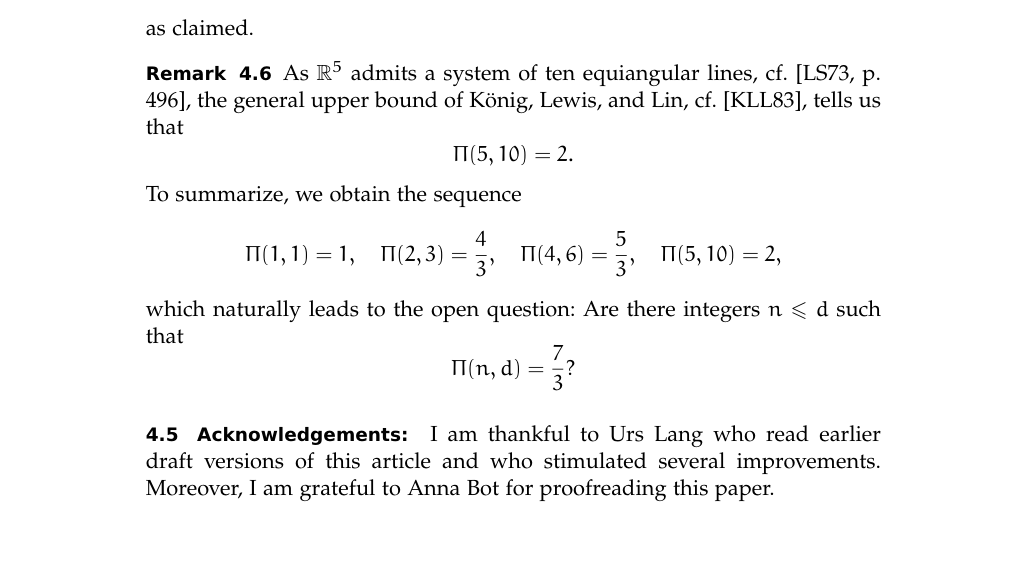
\includegraphics[width=0.92\textwidth]{figures/source_open_question_page24.png}
\caption{Basso, Remark 4.6, where the \(7/3\) question is posed.}
\end{figure}

\section*{KLL Criterion Used}

Basso recalls the theorem of Koenig--Lewis--Lin \cite{KLL1983}:
\[
  \PiRel(n,d)\le
  \Bnd(n,d):=
  \frac nd+\sqrt{(d-1)\frac nd\left(1-\frac nd\right)}.
\]
The equality case is used here in the full-dimensional form also used in the
human review of the original packet: equality is certified by \(d\) distinct
equiangular lines whose representatives span an \(n\)-dimensional Euclidean
space.  This full-dimensional condition is essential.  A lower-dimensional
equiangular configuration embedded into a larger \(\R^n\) is not, by itself,
a KLL equality certificate for \(\PiRel(n,d)\).

\begin{figure}[h]
\centering
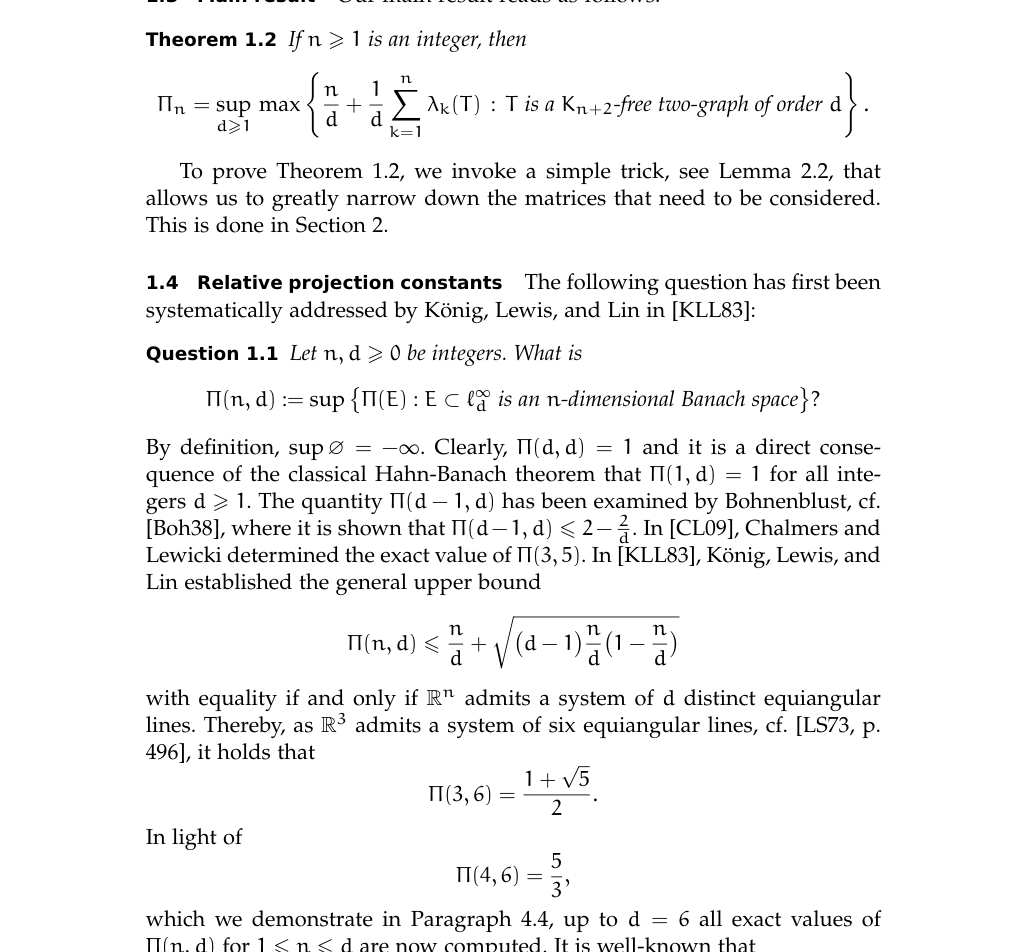
\includegraphics[width=0.92\textwidth]{figures/source_definition_kll_page4.png}
\caption{Basso's definition of \(\Pi(n,d)\) and the quoted
Koenig--Lewis--Lin equality criterion.}
\end{figure}

\section*{Main Outcome}

The corrected systematic principle is the spanning interval principle:
if \(M\) equiangular lines span \(\R^n\), then one gets exact KLL values for
every number \(d\) of lines between \(n\) and \(M\).  This turns the original
\(\PiRel(7,15)=7/3\) observation into the full interval
\[
  \PiRel(7,d)=\Bnd(7,d)\qquad(7\le d\le28),
\]
and Paley conference matrices give infinitely many further intervals
\[
  \PiRel\left(\frac{q+1}{2},d\right)
  =
  \Bnd\left(\frac{q+1}{2},d\right)
  \qquad
  \left(\frac{q+1}{2}\le d\le q+1,\ q\equiv1\pmod4\right).
\]

For Basso's specific value \(7/3\), the KLL upper bound itself reaches
\(7/3\) at exactly two integer pairs:
\[
  (n,d)=(7,15),\qquad (n,d)=(49,51).
\]
Both are sharp.  The first is supplied by the \(E_7\) 28-line configuration.
The second is supplied by the Paley conference matrix for \(q=97\), which
gives \(98\) equiangular lines spanning \(\R^{49}\); a 51-line spanning
subsystem certifies
\[
  \PiRel(49,51)=\frac73.
\]

\section*{Why the Spanning Condition Matters}

It is tempting to use equiangular systems in lower-dimensional subspaces and
then embed them into larger Euclidean spaces.  This would be too strong.  For
example, six equiangular lines in \(\R^3\) can be embedded into \(\R^4\), but
Basso records
\[
  \PiRel(4,6)=\frac53,
\]
whereas the KLL upper bound \(\Bnd(4,6)\) is larger than \(5/3\).  Thus a
mere lower-dimensional embedding cannot be the intended equality condition.
All equality certificates below are therefore full-dimensional: the selected
lines span the relevant \(\R^n\).

\section*{Proof Intuition}

The previous proof used one 15-line subset of a classical 28-line system in
dimension 7.  Since seven lines in that chosen system already form a basis,
one can add any further lines from the same equiangular configuration and keep
a spanning equiangular system.  That gives every \(d\) from 7 to 28 at once.

The same mechanism works for conference matrices.  A symmetric conference
matrix of order \(2n\) yields \(2n\) equiangular lines spanning \(\R^n\), so
every \(d\) between \(n\) and \(2n\) is KLL-exact.  Paley's finite-field
construction gives infinitely many such conference matrices.  Taking
\(q=97\) gives exactly the new \(7/3\) pair \((49,51)\).

\section*{The Spanning Interval Principle}

\begin{theorem}[Spanning interval principle]
Suppose \(\R^n\) contains \(M\) distinct equiangular lines spanning \(\R^n\).
Then, for every integer \(d\) with \(n\le d\le M\),
\[
  \PiRel(n,d)=
  \frac nd+\sqrt{(d-1)\frac nd\left(1-\frac nd\right)}.
\]
\end{theorem}

\begin{proof}
Choose nonzero representatives of the \(M\) lines.  Since the representatives
span \(\R^n\), some \(n\) of them are linearly independent.  Fix those \(n\)
basis lines and add any \(d-n\) further lines from the original equiangular
system.  The selected \(d\) lines remain equiangular and still span \(\R^n\).
The Koenig--Lewis--Lin equality criterion gives the displayed equality.
\end{proof}

\section*{The \(E_7\) Interval}

\begin{corollary}
For every integer \(d\) with \(7\le d\le28\),
\[
  \PiRel(7,d)=
  \frac7d+\sqrt{(d-1)\frac7d\left(1-\frac7d\right)}.
\]
In particular, \(\PiRel(7,15)=7/3\).
\end{corollary}

\begin{proof}
Let
\[
  H=\left\{x\in\R^8:\sum_{i=1}^8 x_i=0\right\}.
\]
For each two-element subset \(A\subset\{1,\ldots,8\}\), define
\[
  v_A=\sum_{i\in A}e_i-\frac14(1,\ldots,1)\in H.
\]
For two such sets \(A,B\),
\[
  \langle v_A,v_B\rangle=|A\cap B|-\frac12.
\]
Thus the 28 lines \(\R v_A\) are equiangular in \(H\cong\R^7\).  The seven
vectors \(v_{\{1,j\}}\), \(2\le j\le8\), form a basis of \(H\): if
\[
  \sum_{j=2}^8 a_jv_{\{1,j\}}=0
\]
and \(A=\sum_{j=2}^8a_j\), then the coordinates \(2,\ldots,8\) give
\(a_j=A/4\) for every \(j\), hence \(A=7A/4\), so all \(a_j=0\).
The spanning interval principle applies.
\end{proof}

\section*{Conference and Paley Intervals}

\begin{theorem}[Conference intervals]
Suppose there is a symmetric conference matrix of order \(2n\).  Then, for
every integer \(d\) with \(n\le d\le2n\),
\[
  \PiRel(n,d)=
  \frac nd+\sqrt{(d-1)\frac nd\left(1-\frac nd\right)}.
\]
\end{theorem}

\begin{proof}
Let \(C\) be a symmetric conference matrix of order \(2n\):
\[
  C_{ii}=0,\qquad C_{ij}\in\{\pm1\}\ (i\ne j),\qquad C^2=(2n-1)I.
\]
Since \(C\) is symmetric, its eigenvalues are \(\pm\sqrt{2n-1}\).  Also
\(\operatorname{tr} C=0\), so the two eigenspaces have the same dimension,
namely \(n\).
The projection
\[
  P=\frac12\left(I+\frac1{\sqrt{2n-1}}C\right)
\]
has rank \(n\), diagonal entries \(1/2\), and off-diagonal entries of common
absolute value \(1/(2\sqrt{2n-1})\).  Hence \(P\) is the Gram matrix of
\(2n\) equiangular lines spanning \(\R^n\).  The spanning interval principle
applies.
\end{proof}

\begin{corollary}[Paley intervals]
Let \(q\) be an odd prime power with \(q\equiv1\pmod4\), and put
\[
  n=\frac{q+1}{2}.
\]
Then, for every integer \(d\) with \(n\le d\le q+1\),
\[
  \PiRel(n,d)=
  \frac nd+\sqrt{(d-1)\frac nd\left(1-\frac nd\right)}.
\]
At the endpoint,
\[
  \PiRel\left(\frac{q+1}{2},q+1\right)=\frac{1+\sqrt q}{2}.
\]
\end{corollary}

\begin{proof}
Let \(\F_q\) be the finite field with \(q\) elements, and let
\(\chi:\F_q\to\{0,\pm1\}\) be the quadratic character.  Index rows and
columns by \(\F_q\cup\{\infty\}\), and define
\[
  C_{\infty,\infty}=0,\qquad
  C_{\infty,x}=C_{x,\infty}=1\quad(x\in\F_q),
\]
\[
  C_{x,x}=0,\qquad
  C_{x,y}=\chi(x-y)\quad(x,y\in\F_q,\ x\ne y).
\]
Since \(q\equiv1\pmod4\), \(\chi(-1)=1\), so \(C\) is symmetric.  The
standard quadratic-character identity
\[
  \sum_{t\in\F_q}\chi((t-a)(t-b))=-1\qquad(a\ne b)
\]
implies \(C^2=qI_{q+1}\).  Hence \(C\) is a symmetric conference matrix of
order \(q+1=2n\).  The conference interval theorem applies.
\end{proof}

\section*{The KLL Route to \(7/3\)}

\begin{lemma}[Fixed target arithmetic]
Fix a rational number \(c>1\).  The integer pairs \(n\le d\) satisfying
\[
  \Bnd(n,d)=c
\]
are finite and are given by the formula
\[
  d=
  \frac{n(n+1-2c)}{n-c^2}
  =
  n+\frac{n(c-1)^2}{n-c^2},
\]
whenever the right-hand side is an integer at least \(n\).
\end{lemma}

\begin{proof}
The equation \(\Bnd(n,d)=c\) is equivalent to
\[
  \sqrt{(d-1)\frac nd\left(1-\frac nd\right)}=c-\frac nd.
\]
Squaring and simplifying gives the displayed formula.  Since \(d\ge n\), the
second expression forces \(n>c^2\).  For \(n>c^2\), the difference
\[
  d-n=\frac{n(c-1)^2}{n-c^2}
\]
is a decreasing function of \(n\) and is bounded.  Hence only finitely many
integer values of \(m=d-n\) can occur.  For each such \(m\), the equation
\[
  m(n-c^2)=n(c-1)^2
\]
determines at most one value of \(n\).  Therefore only finitely many integer
pairs can occur.
\end{proof}

\begin{theorem}
The integer pairs \(n\le d\) for which the Koenig--Lewis--Lin upper bound
\(\Bnd(n,d)\) is exactly \(7/3\) are precisely
\[
  (n,d)=(7,15)\quad\text{and}\quad(n,d)=(49,51).
\]
For both pairs the bound is sharp.  Therefore
\[
  \PiRel(7,15)=\PiRel(49,51)=\frac73.
\]
\end{theorem}

\begin{proof}
For \(c=7/3\), the fixed-target formula gives
\[
  d=n+\frac{16n}{9n-49}.
\]
As \(d\ge n\) and \(d\ne n\), put \(m=d-n\ge1\).  Then
\[
  (9m-16)n=49m.
\]
The denominator must be positive, so \(m\ge2\), and the condition \(n\ge6\)
forces \(m\le19\).  Also \(9m-16\) divides \(49m\), hence it divides
\[
  9(49m)-49(9m-16)=784.
\]
Among positive divisors \(r\) of \(784\) with \(r=9m-16\) and \(2\le m\le19\),
only \(r=2\) and \(r=56\) occur.  These give
\[
  (m,n,d)=(2,49,51)\quad\text{and}\quad(8,7,15).
\]

The pair \((7,15)\) is sharp by the \(E_7\) interval.  For \((49,51)\), use
the Paley construction with \(q=97\).  Since \(97\) is prime and
\(97\equiv1\pmod4\), it gives \(98\) equiangular lines spanning
\(\R^{49}\).  The spanning interval principle gives
\[
  \PiRel(49,51)=
  \frac{49}{51}+
  \sqrt{50\cdot\frac{49}{51}\cdot\frac2{51}}
  =
  \frac{49}{51}+\frac{70}{51}
  =
  \frac73.
\]
\end{proof}

\begin{remark}
This theorem classifies the pairs for which the KLL upper bound itself equals
\(7/3\).  It is not a full classification of all conceivable pairs satisfying
\(\PiRel(n,d)=7/3\), because a pair with \(\Bnd(n,d)>7/3\) could in principle
have exact value \(7/3\) by some non-KLL mechanism.
\end{remark}

\section*{Large Classical Intervals}

The same spanning interval principle turns every known full-dimensional
equiangular-line system into exact relative projection constants.  In
particular, the classical Gerzon-sharp systems in dimensions \(2,3,7,23\)
give
\[
  \PiRel(2,d)=\Bnd(2,d)\qquad(2\le d\le3),
\]
\[
  \PiRel(3,d)=\Bnd(3,d)\qquad(3\le d\le6),
\]
\[
  \PiRel(7,d)=\Bnd(7,d)\qquad(7\le d\le28),
\]
and, using the classical 276 equiangular lines in \(\R^{23}\),
\[
  \PiRel(23,d)=\Bnd(23,d)\qquad(23\le d\le276).
\]
The last interval is included as a literature-backed application rather than
as a new construction in this note; the 276-line system is standard in the
equiangular-lines literature \cite{LS1973,LinYu2018}.

\section*{A Small ``Thirds Ladder''}

The fixed-target arithmetic can be applied to neighboring values \(k/3\).
The table below lists selected KLL-bound candidates that are certified by the
spanning equiangular systems used above.  It is not a classification table
for these other values; its role is to show that Basso's \(7/3\) question is
part of a broader exact-value mechanism.

\[
\begin{array}{c|l|l}
\text{value} & \text{certified pairs }(n,d) & \text{source}\\
\hline
4/3 & (2,3) & \text{simplex}\\
5/3 & (5,6) & \text{simplex or Paley }q=9\\
2 & (5,10) & \text{Paley }q=9\\
7/3 & (7,15),(49,51) & E_7;\ \text{Paley }q=97\\
3 & (13,26),(15,25),(21,28) & \text{Paley }q=25,29,41\\
3 & (27,33),(45,50) & \text{Paley }q=53,89\\
\end{array}
\]

\section*{Literature Exploration and Further Tools}

The original source has a later erratum \cite{BassoErratum2024}.  The erratum
concerns an error in Lemma 3.1 and a different part of the computation of
maximal projection constants.  The present note uses the KLL/equiangular-line
criterion quoted in Section 1.4 of the original paper, not the affected lemma.

The equiangular-line side has much more raw material than is used above.
Lemmens--Seidel \cite{LS1973} is the classical reference for equiangular
lines, conference matrices, and the low-dimensional exceptional systems.
Greaves--Koolen--Munemasa--Szollosi \cite{GKMS2014} develop Seidel-matrix and
computational tools for equiangular lines in Euclidean spaces.  Lin--Yu
\cite{LinYu2018} gives modern structural context around the
Lemmens--Seidel conjecture and the special Gerzon-sharp dimensions.  Fixed
angle asymptotics, as in Jiang--Tidor--Yao--Zhang--Zhao
\cite{JiangTidorYaoZhangZhao2021}, suggest a possible source of broad lower
bounds, though exact KLL equality still requires actual full-dimensional
finite equiangular systems.  Other equiangular tight frame constructions,
such as the Tremain and Steiner/Hadamard families studied by
Fickus--Jasper--Mixon--Peterson \cite{FJMP2016}, are promising future inputs
for more exact \(\PiRel(n,d)\) intervals.

For a full \(7/3\) classification, the main missing ingredient would be a way
to rule out non-KLL mechanisms for pairs whose KLL upper bound is larger than
\(7/3\).  Basso's two-graph/eigenvalue framework and linear-programming
formulations of relative projection constants look like the relevant tools,
but they are outside the short equiangular argument of this note.

\section*{Verification Notes}

The script \texttt{code/verify\_systematic\_families.py} checks the finite
certificates and arithmetic used in this packet.

First, it verifies with exact rational arithmetic that the \(E_7\) model gives
28 equiangular lines spanning \(\R^7\), and that the interval
\(7\le d\le28\) can be selected so as to remain spanning.  It also checks that
the \(d=15\) KLL value is exactly \(7/3\).

Second, it verifies the integer search behind the KLL-bound equation
\(\Bnd(n,d)=7/3\), recovering only \((7,15)\) and \((49,51)\).

Third, it constructs Paley conference matrices for all primes
\(q\equiv1\pmod4\) up to 100 and verifies \(C^2=qI\).  For \(q=97\), it also
checks with exact arithmetic over \(\mathbb Q(\sqrt{97})\) that the first 51
Paley lines have Gram rank 49, giving an explicit spanning certificate for
\(\PiRel(49,51)=7/3\).

Finally, it verifies the sample thirds-ladder entries displayed above.

\section*{Limitations and Novelty}

The packet does not claim a new equiangular-line construction.  Its
contribution is the translation: known full-dimensional equiangular-line
systems give intervals of exact relative projection constants.  The most
concrete payoff for Basso's question is
\[
  \PiRel(7,15)=\PiRel(49,51)=\frac73,
\]
together with a proof that these are the only KLL-bound equality points at
the value \(7/3\).

The result stops short of a complete classification of \(\PiRel(n,d)=7/3\).
Such a classification would need control over possible non-KLL equality
mechanisms when the KLL upper bound is strictly larger than \(7/3\).

\section*{Human Review Recommendation}

Review should focus on four points.  First, confirm the exact full-dimensional
form of the Koenig--Lewis--Lin equality criterion.  Second, check the spanning
interval principle.  Third, check the arithmetic classification of KLL-bound
equality at \(7/3\).  Fourth, check the Paley \(q=97\) spanning certificate
for the new pair \((49,51)\).

\begin{thebibliography}{10}

\bibitem{Basso2019}
G. Basso,
\emph{Computation of maximal projection constants},
arXiv:1901.07866, 2019.
\url{https://arxiv.org/abs/1901.07866}

\bibitem{BassoErratum2024}
G. Basso,
\emph{Erratum to ``Computation of maximal projection constants''},
arXiv:2402.06672, 2024.
\url{https://arxiv.org/abs/2402.06672}

\bibitem{KLL1983}
H. Koenig, D. R. Lewis, and P.-K. Lin,
\emph{Finite dimensional projection constants},
Studia Math. 75 (1983), 341--358.

\bibitem{LS1973}
P. W. H. Lemmens and J. J. Seidel,
\emph{Equiangular lines},
J. Algebra 24 (1973), 494--512.

\bibitem{Paley1933}
R. E. A. C. Paley,
\emph{On orthogonal matrices},
J. Math. Phys. 12 (1933), 311--320.

\bibitem{GKMS2014}
G. R. W. Greaves, J. H. Koolen, A. Munemasa, and F. Szollosi,
\emph{Equiangular lines in Euclidean spaces},
arXiv:1403.2155, 2014.
\url{https://arxiv.org/abs/1403.2155}

\bibitem{LinYu2018}
Y.-T. Lin and W.-H. Yu,
\emph{Equiangular lines and the Lemmens-Seidel conjecture},
arXiv:1807.06249, 2018.
\url{https://arxiv.org/abs/1807.06249}

\bibitem{JiangTidorYaoZhangZhao2021}
Z. Jiang, J. Tidor, Y. Yao, S. Zhang, and Y. Zhao,
\emph{Equiangular lines with a fixed angle},
Ann. of Math. 194 (2021), 729--743.
\url{https://arxiv.org/abs/1907.12466}

\bibitem{FJMP2016}
M. Fickus, J. Jasper, D. G. Mixon, and J. Peterson,
\emph{Tremain equiangular tight frames},
arXiv:1602.03490, 2016.
\url{https://arxiv.org/abs/1602.03490}

\end{thebibliography}

\end{document}
